\documentclass[12pt]{article}
\usepackage[utf8]{inputenc}
\usepackage{graphicx} %Paquete utilizado para insertar imágenes en el documento
\title{Insertar imágenes}
\author{Curso de introducción a LaTeX}
\begin{document}
\maketitle

\section{Lorem ipsum dolor sit}

%Incluir un gráfico simple:
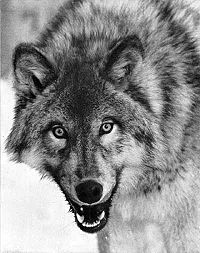
\includegraphics{canis} 

Lorem ipsum dolor sit amet, ut amet nec massa tincidunt, auctor dolor, pharetra at massa, quis sem netus amet. Auctor amet nec. Sollicitudin quis. Magna purus vehicula mauris lectus ultrices amet, duis dolor in ut feugiat ultricies ridiculus, id fusce malesuada quisque morbi varius, bibendum ante duis vitae aliquam ut sed, integer tellus habitasse nec lectus fugiat posuere. Massa venenatis tempus ut ut donec, conubia sapien luctus eget varius velit. Mi ipsum tellus, mauris eleifend.

% Centrar un gráfico importado:
\begin{center}
	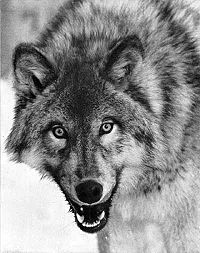
\includegraphics{canis}
\end{center}

Magna ipsum felis vel mauris hendrerit lobortis, suspendisse tellus, metus nec massa nibh wisi, pede nec ullamcorper facilisis pharetra, pulvinar lectus arcu nulla faucibus et metus. Vestibulum vulputate dolor velit, blandit duis dis, placerat urna euismod, mauris sed nibh dolorem dui, nec pellentesque rhoncus porta. Pellentesque ipsum, in id, ultricies proin tellus euismod metus, rhoncus faucibus facilisi suspendisse nulla proin, dapibus placerat est quis faucibus dignissim. 

%Hay un problema cuando el gráfico es muy grande:
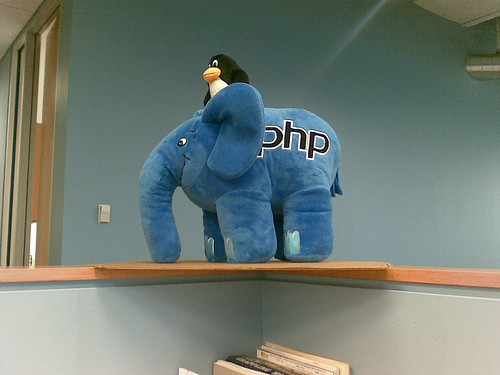
\includegraphics{php}

\section{At id laoreet quam bibendum}

At id laoreet quam bibendum. Arcu mauris at at, nam volutpat eu. Delectus nostra debitis luctus posuere ut, ut suspendisse arcu nec molestie pede et, velit nec elementum justo elit sed enim. Nunc praesent vestibulum fusce aliquam eros quis, enim nulla, et iste cursus iaculis euismod accusantium, ac nibh dui vehicula, pede viverra eleifend. Lorem libero felis ante ut convallis rutrum. Orci luctus etiam, libero ut sem dignissim condimentum pharetra, neque erat turpis, purus tempor euismod feugiat libero amet auctor. 

% Y podemos solucionarlo ajustando sus dimensiones:
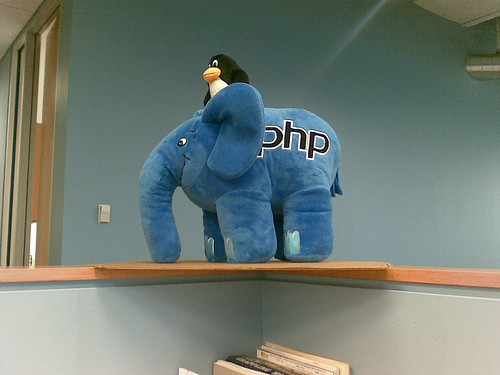
\includegraphics[width=100px, height=80px]{php}

Nonummy cursus aliquip rutrum porta, viverra ac sit viverra ornare. Facilisis aliquam leo eu id. Proin porttitor amet turpis congue sequi. Augue eros in wisi amet nec eu, id consectetuer voluptatibus et, dolor pede eget amet. Quam lectus vivamus non enim, scelerisque feugiat feugiat magna sit lacus, justo commodo. Ut ac malesuada, feugiat rutrum, amet cum ullamcorper dictumst, amet ligula donec vel mi tristique est, eros condimentum leo. Semper vestibulum eros mauris enim mauris, mauris massa. 

% También podemos ajustar una imagen escalándola:
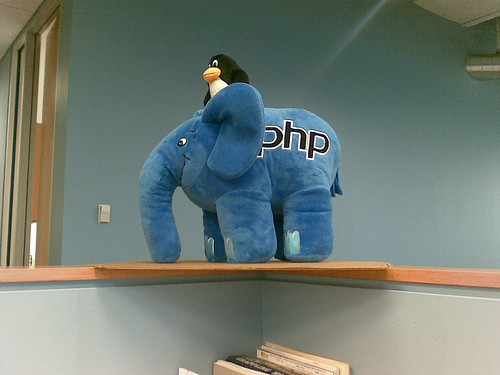
\includegraphics[scale=0.5]{php}

\section{In morbi non}
In morbi non purus magna posuere sodales, feugiat  atque est. Urna nunc amet consequat hac, consequat luctus et magnis per dui, nunc tempor, sed venenatis. Neque urna eu, nam sed elit duis. Vestibulum purus mauris vestibulum lectus pede mollis, phasellus vestibulum justo montes, aliquam eget id semper nibh magna, a donec eget id, elit dignissim tortor blandit mauris vivamus lectus. Porttitor cras, ut libero nulla sapien erat curabitur eleifend. Blandit quis.


% Otra forma es ajustar sólo en ancho de la imagen al tamaño del área imprimible del documento:
\noindent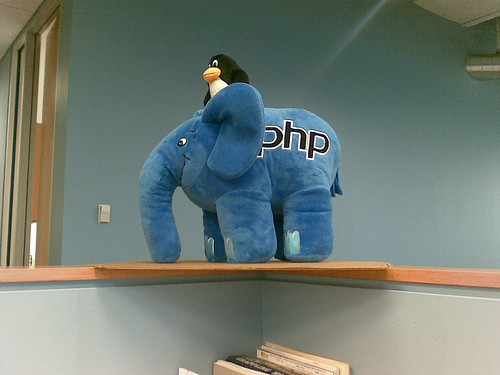
\includegraphics[width=\textwidth]{php}

Purus ante, mauris nec lacus quis vestibulum purus convallis, sed aliquet pede libero nibh. Eget magna neque mi, ipsum cras consectetuer, est nullam massa dui lacus, tincidunt nec, at suspendisse. Id nulla vestibulum, turpis suscipit amet. Cum sagittis praesent, quam mauris ac tincidunt vel. Scelerisque pellentesque nibh tristique et sed, donec nulla laoreet.

\section{Vulputate vel vulputate}

Nunc praesent vestibulum fusce aliquam eros quis, enim nulla, et iste cursus iaculis euismod accusantium, ac nibh dui vehicula, pede viverra eleifend. Lorem libero felis ante ut convallis rutrum. Orci luctus etiam, libero ut sem dignissim condimentum pharetra, neque erat turpis, purus tempor euismod feugiat libero amet auctor. 

% O ajustarla al ancho de la línea del documento:
\noindent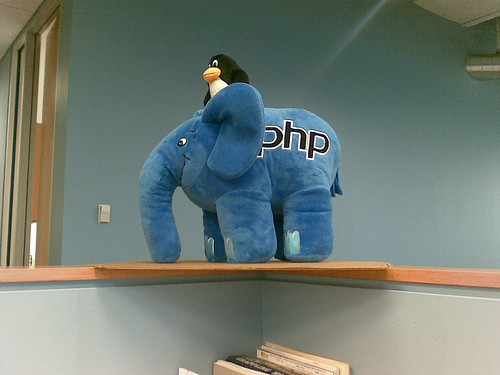
\includegraphics[width=\linewidth]{php}

Vestibulum purus mauris vestibulum lectus pede mollis, phasellus vestibulum justo montes, aliquam eget id semper nibh magna, a donec eget id, elit dignissim tortor blandit mauris vivamus lectus. Porttitor cras, ut libero nulla sapien erat curabitur eleifend. Blandit quis.

% Ajustando también ese ancho a un 70%:
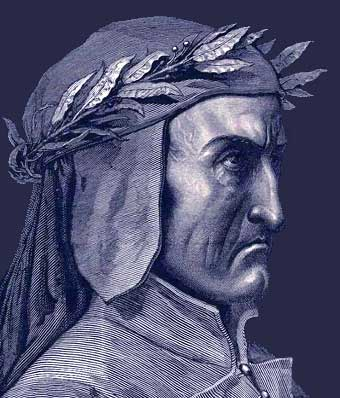
\includegraphics[width=0.7\linewidth]{img/dante}

In vitae nisl arcu ut varius ut, erat a pellentesque iaculis lacus. Sem eget praesent sapien dictum pretium rutrum. Vulputate vel vulputate, justo diam amet enim vestibulum bibendum dictum, sapien praesent mauris, amet semper vitae quam vitae justo et.

% También podemos importar gráficos vectoriales en formato PDF:

\includegraphics[width=0.7\linewidth]{img/cicimar}

Augue eros in wisi amet nec eu, id consectetuer voluptatibus et, dolor pede eget amet. Quam lectus vivamus non enim, scelerisque feugiat feugiat magna sit lacus, justo commodo. Ut ac malesuada, feugiat rutrum, amet cum ullamcorper dictumst, amet ligula donec vel mi tristique est, eros condimentum leo. Semper vestibulum eros mauris enim mauris, mauris massa. 

\section{Mi imagen}

Ahora, prueba introducir una imagen por ti mismo (puedes utilizar el asistente para Insertar Gráficos localizado en la barra de tareas):

\begin{center}
	
\includegraphics[width=0.7\linewidth]{img/Escudo-UPIICSA.png}
\end{center}



\end{document}
